\part{Modèle algébrique}
Pour manipuler toutes les données des systèmes observés, nous avons choisi de décrire un langage d'interrogation unique. Afin d'avoir des définitions précises des sémantiques des requêtes, nous avons décidé de faire le langage algébrique Astral. Dans cette partie, nous détaillons ce langage et ses capacités. Nous consacrons un chapitre à l'ensemble de ses définitions (des n-uplets jusqu'aux opérateurs). Puis, nous comparons cette algèbre avec les approches existantes et nous présentons quelques résultats d'équivalence de requêtes.

\begin{savequote}[6cm]
<< Don't you use your fancy mathematics to muddle the issue! >>
\qauthor{Applejack}
\end{savequote}

\chapter{Astral : Modèle théorique de requêtes continues}
\chaptertoc

La gestion de flux de données est un domaine dérivé de la gestion de base de données relationnelles. Afin de pouvoir définir un langage de requête uniforme pour pouvoir interroger autant les flux que les relations, il nous faut définir un modèle algébrique précis. Nous accorderons comme importance primordiale le déterminisme du modèle. En effet, plusieurs formalisations ont permis dans certains cas le fait de faire des choix non-déterministe. Cet aspect apporte un flou sur les réponses aux requêtes. Nous souhaitons formaliser exactement les bases de l'algèbre afin de pouvoir fédérer tous les modèles existants.

Nous développerons dans ce chapitre les fondations de notre algèbre : \textit{Astral} (\textit{Advanced Stream Algebra}). Cette algèbre reprend des bases théoriques développés dans \textit{STREAM}~\cite{Arasu:stream} (lui même basé sur le modèle relationnel) tout en précisant des concepts clés pour en améliorer l'expressivité et la clareté. Ce chapitre définit les concepts primitifs tels que les n-uplets, les flux, relations ainsi que la notion de requête dans la section~\ref{sec:contrib:astral:definitions}. Par la suite, nous présenterons les opérateurs : tout d'abord ceux issus de l'algèbre relationnel (section~\ref{sec:contrib:astral:relationnel}), puis ceux plus spécifiques à la gestion de flux (section~\ref{sec:contrib:astral:flux}). Enfin, nous investigerons l'influence de l'instant de début d'une requête sur son fonctionnement en section~\ref{sec:contrib:astral:transposabilite}. Puis, nous concluerons par une synthèse de ce modèle en section~\ref{sec:contrib:astral:conclusion}.

\section{Définitions générales}
\subsection{N-uplets et identifiants}Aliquam dictum risus ac nulla rutrum molestie. Proin at erat urna, nec dignissim velit. Nullam fringilla augue at est vulputate tincidunt. Nam non condimentum tellus. Aenean orci magna, accumsan rutrum faucibus eget, pretium adipiscing justo. Donec dignissim faucibus scelerisque. Aenean adipiscing tellus sed nulla euismod tempus eleifend justo molestie. Quisque in ligula quis velit condimentum pharetra.

Ut et est arcu. Fusce at dapibus augue. Vestibulum porta pretium vestibulum. Duis aliquam aliquam mattis. Praesent dapibus sem vel tellus rhoncus non posuere nunc egestas. Ut sit amet mauris tortor, sit amet tristique lacus. Pellentesque porta faucibus vestibulum. Curabitur non quam urna, et vulputate eros. 
\begin{defi}[n-uplet]
    Un n-uplet est une fonction partielle de l'ensemble des attributs vers l'espace des valeurs. Le domaine de cette fonction est appellé le schéma du n-uplet.
\end{defi}
Lorem ipsum dolor sit amet, consectetur adipiscing elit. Cras nulla arcu, ullamcorper quis malesuada et, vestibulum sed lectus. Cras volutpat, nulla eu consectetur adipiscing, leo ligula feugiat sem, eget suscipit lacus nunc eget mauris. Aenean posuere lobortis augue sit amet elementum. Integer arcu leo, varius et elementum eu, vehicula sed turpis. Donec et quam quam, sit amet lobortis orci. Cum sociis natoque penatibus et magnis dis parturient montes, nascetur ridiculus mus. Etiam eu lorem erat, at ornare diam.

Donec porttitor commodo consequat. Curabitur pharetra purus ac tellus viverra varius. Vivamus tincidunt, quam at adipiscing pharetra, nunc mi blandit nulla, quis porttitor tellus ligula in erat. Donec auctor enim vel lorem aliquam vestibulum. Phasellus sit amet sollicitudin arcu. Etiam interdum dictum leo, ac malesuada lorem ultricies id. Nam sit amet orci sed mauris lobortis vestibulum. Quisque lobortis, erat at venenatis scelerisque, orci lectus gravida massa, id laoreet dolor augue a metus. 
\begin{defi}[Identifiant physique]
    L'identifiant physique d'un n-uplet $s$ est un élément de l'espace des identifiants $\I$ isomorphe à $\N$. Le nom d'attribut de cet identifiant sera noté $\varphi$ et $s(\varphi)$ désigne la valeur de l'identifiant de $s$.
\end{defi}

    L'identifiant physique d'un n-uplet $s$ est un élément de l'espace des identifiants $\I$ isomorphe à $\N$. Le nom d'attribut de cet identifiant sera noté $\varphi$ et $s(\varphi)$ désigne la valeur de l'identifiant de $s$.

\begin{defi}[Séquence d'n-uplet]
    Un ensemble dénombrable d'n-uplets $TS$ est une séquence si et seulement si : 
    \begin{itemize}
     \item Tout n-uplet de $TS$ partage le même schéma $A$ contenant $\varphi$.
     \item $\forall s,s' \in TS^2$, $s\neq s' \equ s(\varphi) \neq s'(\varphi)$
    \end{itemize}

    Une séquence est donc naturellement totalement ordonné par son identifiant physique.
\end{defi}
Aliquam dictum risus ac nulla rutrum molestie. Proin at erat urna, nec dignissim velit. Nullam fringilla augue at est vulputate tincidunt. Nam non condimentum tellus. Aenean orci magna, accumsan rutrum faucibus eget, pretium adipiscing justo. Donec dignissim faucibus scelerisque. Aenean adipiscing tellus sed nulla euismod tempus eleifend justo molestie. Quisque in ligula quis velit condimentum pharetra.

Ut et est arcu. Fusce at dapibus augue. Vestibulum porta pretium vestibulum. Duis aliquam aliquam mattis. Praesent dapibus sem vel tellus rhoncus non posuere nunc egestas. Ut sit amet mauris tortor, sit amet tristique lacus. Pellentesque porta faucibus vestibulum. Curabitur non quam urna, et vulputate eros. 

\begin{prop}[Timestamp]
    L'espace temps $\T$ est un corps totalement ordonné et isomorphique à $\R$. 

    Un \textit{timestamp} est un élément de $\T$.
\end{prop}


\begin{thm}[Identifiant de batch]
    Un identifiant de batch est un élément de l'ensemble $\TN$ totalement ordonné par lexicographie.
\end{thm}

\begin{coro}[Flux]
    Un flux est un couple $(S,\BS)$ tel que :
    \begin{itemize}
        \item $S$ est une séquence d'n-uplet potentiellement infinie possédant un schéma contenant l'attribut spécial $\t$.
        \item $\BS$ est une fonction $S\mapsto \TN$ définissant le batch d'appartenance d'un n-uplet
    \end{itemize}
\end{coro}


\section{Héritages du modèle relationnel}
La définition de relation temporelle que nous avons exposé comporte la notion de séquence d'n-uplet. Cette notion est certes proche des relations classiques mais possède un point majeur supplémentaire étant l'ordre. Dans cette section, nous verrons comment réutiliser les opérateurs de l'algèbre relationnelle.

\subsection{Opérateurs unaires simples}
Tout d'abord explorons le domaine des opérateurs unaires relationnels : sélection, projection et renommage. Comme ces opérateurs sont agnostiques de l'ordre dans lesquels sont les n-uplets, le principe de l'héritage est d'appliquer les définitions sur l'évaluation instantanée de la relation.

Par exemple, notons la sélection relationnelle classique $\Sigma$. Alors, pour un batch $b$ quelconque, l'expression suivante : $\Sigma(R(b))$, exprime bien la sélection des n-uplets. Ainsi l'application de l'opérateur relationnel standard sur le batch présent permet de définir la sélection (def~\ref{def:selection}). L'identifiant physique n'est pas altéré donc l'ordre ne l'est pas non plus.
\begin{defi}[Sélection]\label{def:selection}
Soit $R$ une relation temporelle,

Soit $c$ une expression booléenne applicable sur tout n-uplet de $R$,

Alors la sélection est définie comme suit :
$$\sigma_{c}(R) : b \mapsto \{s\in R(b), c(s)\} = \Sigma_c(R(b))$$
\end{defi}

Nous pouvons remarquer d'ores et déjà que la définition d'inclusion de requête est directement appliquable à la sélection (en prenant pour fonction d'extraction l'identité).
\begin{prop}[Inclusion de la sélection]
Soit $R$ une relation temporelle, et $c$ une condition de sélection, alors $\sigma_c R \subseteqq R$
\end{prop}

La projection et le renommage se définissent de façon similaire. Toutefois, il existe des cas pouvant altérer l'identifiant physique. Par exemple, la projection sur des attributs ne comprennant pas $\varphi$ le supprimerait. Nous instaurons donc des règles supplémentaires (def~\ref{projection}) pour éviter ces cas. De façon similaire, nous pourrions définir l'opérateur d'évaluation d'expressions $e_f^c$ permettant d'évaluer une expression $f$ dont le résultat serait placé dans l'attribut $c$.
\begin{defi}[Projection et renommage]\label{def:projection}
La projection $\Pi_p$ et le renommage $\rho_{b/a}$ sont défini par héritage de l'algèbre relationnelle à l'exception de ces deux règles :
\begin{itemize}
\item Une projection $\Pi_p$ est strictement égale à $\Pi_{p\cup \{\varphi\}}$
\item Le renommage $\rho_{b/\varphi}$ correspond a une copie de $\varphi$ dans $b$.
\end{itemize}
\end{defi}

Nous avons donc réussi à appliquer les définitions des 3 premiers opérateurs de l'algèbre relationnelle dans notre contexte. Il nous faut maintenant explorer les opérateurs binaires, en commençant par la jointure.

\subsection{Produit cartésien}
La contrainte de l'ordre commence à se faire pesante dans le cadre des opérations binaires. En effet, il nous faut établir un ordre strict sur la séquence d'n-uplets résultants du produit des deux relations. Il est important de noter que cette notion de séquence d'n-uplet est primordiale même pour les relations temporelles (voir notamment les \textit{streamers} def~\ref{def:streamers}).
\begin{example}
\end{example}
\section{Opérateurs de flux}
L'avantage de la gestion de flux est de pouvoir gérer la dynamique des données via des opérateurs dédiés. Astral est construite sur la sémantique a deux concepts, il nous faut donc définir les opérateurs flux vers relation (fenêtres) et relation vers flux (streamers). Puis, nous définirons et explorerons des opérateurs spécifiques à la gestion de flux étant : la gestion des modifications des relations et des \textit{batchs}.
\subsection{Fenêtres}
L'opérateur de fenêtre est un des opérateurs les plus étudiés dans la littérature. Toutefois, son comportement est encore flou sur certains points. La formalisation de son fonctionnement permettra donc une meilleure compréhension.
\subsubsection{Association position-\textit{batch}}
Avant de définir formellement l'opération de fenêtrage, nous avons besoin d'un outil pour gérer l'association entre la position d'un n-uplet et de son \textit{batch}. La fonction $\tau_S$ définit cette association. 
\begin{defi}[Fonction position-\textit{batch}]\label{def:tau}
    Soit $S$ un flux,

    La fonction $\tau_S : \N\cup\{-1\}\to \TN$ est la fonction associant un entier à l'identifiant de \textit{batch} du seul n-uplet présent à cette position.

    Par convention, $\tau_S(-1)=(t_0,0)$.
\end{defi}

Par corollaire de l'hypothèse fondamentale~\ref{hyp:ordres}, la fonction $\tau_S$ est donc croissante non-stricte. Ainsi, il est possible de définir une pseudo inverse $\rtau_S$ capable de donner une position (la maximale en l'occurence) pour un \textit{batch} donné.
\begin{coro}[Fonction pseudo-inverse $\tau$]
    Soit $S$ un flux,

    La pseudo-inverse $\rtau_S:\TN\to \N\cup\{-1\}$ existe et correspond à la plus grande position du \textit{batch} donné en entrée. Si aucun \textit{batch} n'existe, le plus proche est utilisé. Formellement, $$\forall b \in \TN, \qquad \tau_S^{-1}(b) = \sum_{n=-1}^{+\infty} n \indic_{[\tau_S(n),\tau_S(n+1)[}(b)$$
\end{coro}

De par sa nature, la fonction $\tau$ et sa pseudo-inverse partagent des propriétés intéressantes que nous pourrons réutiliser lors de démonstrations formelles.
\begin{prop}[Propriétés de $\tau$]
    Soit $S$ un flux, alors les propriétés suivantes sont correctes :
    \begin{eqnarray*}
        t_0 & \leq & \tau_S(0) \\
        \tau_S(\tau_S^{-1}(b)) & \leq & b \\
        n & \leq & \tau_S^{-1}(\tau_S(n))
    \end{eqnarray*}

    De plus, si $\exists s \in S$, $\BS(s)=b$, alors $\tau_S(\tau_S^{-1}(b)) = b$.
\end{prop}
\subsubsection{Description de séquences de fenêtres}
Afin de se rapproche le plus possible d'un aspect déclaratif, nous souhaitons décorréler l'opérateur de fenêtre en deux objets mathématiques : la description et l'opérateur exécutable. Ce dernier prendra une description en argument pour pouvoir représenter la relation temporelle résultante. Le principe des descriptions de séquences de fenêtres est assez simples, il suffit de décrire deux bornes évoluant de manière discrête, et un taux d'évaluation de ces bornes.

\begin{defi}[Description de Séquence de Fenêtre (DSF)]
    Soient $\D$ et $\D'$ pouvant être $\T$ ou $\N$, une description de séquence de fenêtre (DSF) est un triplet $(\alpha,\beta,r)$ tel que :
\begin{itemize}
    \item $r \in \D$ est le taux d'évaluation des bornes de la fenêtre
    \item $\alpha$ et $\beta$ sont deux fonction de $\N\to D'$ représentant l'évolution des bornes.
\end{itemize}

$\alpha(j)$ et $\alpha(j)$ définissent les $j\eme$ valeures des bornes. La première étant donnée pour $j=0$. Ces fonctions se doivent de vérifier les propriétés suivantes (en considérant $\D=\D'=\T$) :
$$\forall j \in \N, \begin{cases} \alpha(j) \leq \beta(j) & \textrm{le début est avant la fin}\\ \alpha(j) \geq t_0 & \textrm{le début existe} \\ \beta(j) \leq jr + \beta(0) & \textrm{la fin est accessible} \end{cases}$$
    Les conditions pour les autres cas pour $\D$ et $\D'$ sont évidentes par application des fonctions $\tau_S$ et $\tau_S^{-1}$.
\end{defi}

\begin{example}
    Nous souhaitons relever tous les $100$ relevés de charge processeur, les $10$ derniers relevés. Dans ce cas, nous souhaitons obtenir une séquence de fenêtres positionnelles générées tous les $100$ n-uplets ($r=100\in \N$). Nous appliquons des bornes positionnelles donc $\alpha,\beta \in (\N\to\N)^2$. La première fenêtre couvrira du $91\eme$ n-uplet au $100\eme$. Ainsi : $\alpha(0) = 91$ et $\beta(0) = 100$. L'évolution des bornes étant linéaire, nous avons donc :
\begin{eqnarray*}
 \alpha(j) &=& 100j+91\\
 \beta(j) &=& 100j + 100\\
 r & = & 100
\end{eqnarray*}
\end{example}

La création de fenêtre nécessite l'association entre les n-uplets du flux et le numéro de fenêtre décrit dans la \textit{DSF}. Pour cela, nous utilisons une \textit{fonction d'attente} utilisant les identifiants de \textit{batch}. Cette fonction donne le rang de la dernière fenêtre au moment indiqué par le batch. Le terme \textit{attente} est lié au fait que l'évaluateur devra attendre avant le prochain changement de $\gamma$.
Nous retrouvons dans cette fonction le caractère \textit{bloquant} des fenêtres.
\begin{defi}[Fonction d'attente $\gamma$]
    Soit $S$ un flux, soit $(\alpha,\beta,r)$ une DSF,

    La fonction d'attente de la DSF est une fonction $\TN \to \N$ associant un identifiant de \textit{batch} à l'identifiant de la dernière fenêtre complétée.
\begin{itemize}
 \item  Si $r\in\T$, cette fonction est définie par $\gamma : (t,i) \mapsto \left\lfloor \frac{t-\beta(0)}{r} \right\rfloor$.
 \item  Si $r\in\N$, cette fonction est définie par $\gamma : (t,i) \mapsto \left\lfloor \frac{\rtau_S(t,i)-\beta(0)}{r} \right\rfloor$.
\end{itemize}
\end{defi}
\begin{example}
    En reprenant l'exemple précédent, après simplification nous obtenons : $$\gamma(b) = \left\lfloor \frac{\rtau_S(b)}{100}\right\rfloor-1.$$
    Si nous supposons que le flux produit un n-uplet par seconde (ainsi, $\rtau_S(t,i) = \lfloor t/1s \rfloor$) : alors $\gamma(1024s,0) = \left\lfloor \frac{1024}{100}\right\rfloor-1 = 9$. Nous avons donc bien la $10\eme$ fenêtre ($j=9$) comme la dernière fenêtre créée à ce moment.
\end{example}

\subsubsection{L'opérateur}
Il devient désormais possible de définir un opérateur permettant  de générer une relation temporelle à partir d'un flux donné. Cette relation temporelle gère ses changements d'état grâce à la fonction $\gamma$. De manière générale, une DSF peut être ramenée simplement à une expression plus générale $(\alpha,\beta,\gamma)$ ce que nous utiliserons pour la définition de séquence de fenêtres.
\begin{defi}[Opérateur de Séquence de Fenêtres]
	Soit $S$ un flux et $(\alpha, \beta, \gamma)$ une description de séquence,
	
	L'opérateur de séquence de fenêtres est défini par : $\forall b \in \TN$, 
	\begin{itemize}
		\item Si $\gamma(b) \geq 0$, 
		\begin{itemize}
			\item Si la description possède des bornes temporelles :
			$$S[\alpha,\beta,\gamma](b) = \left\{s\in S, \ (\alpha(\gamma(b)),0)\leq \BS(s) \leq (\beta(\gamma(b)),i)\right\}$$
			\item Si la description possède des bornes positions :
			$$E(b) = \left\{s\in S, \ \tau_S(\alpha(\gamma(b)))\leq \BS(s) \leq \tau_S(\beta(\gamma(b)))\right\}$$
			$$S[\alpha,\beta,\gamma](b) = \{s \in E(b) / (\#E(b) - \pos_{E(b)}(s)) \leq \beta(\gamma(b)) - \alpha(\gamma(b))$$
		\end{itemize}
		\item Si $\gamma(b) <0$ alors $S[\alpha,\beta,\gamma](b) = \emptyset$
	\end{itemize}
\end{defi}

Plusieurs remarques peuvent être formulées sur cette définition. Tout d'abord, les expressions sont différentes si les bornes sont positionnelles ou temporelles. Pour les fenêtres temporelles, l'opérateur inclue les n-uplets dont l'identifiant de \textit{batch} s'étend :
\begin{itemize}
	\item[\textbf{depuis}] le premier \textit{batch} de la fenêtre : $(\alpha(\gamma(t,i)),0)$, i.e. ceux dont le \textit{timestamp} est supérieur à la borne inférieur.
	\item[\textbf{jusqu'au}] dernier \textit{batch} de la fenêtre : $(\beta(\gamma(t,i)),i)$. Ce qui correspond au $i\eme$ \textit{batch} ayant le \textit{timestamp} inférieur ou égal à la borne.
\end{itemize}
Il est important de voir que $S[\alpha,\beta,\gamma]$ pourra changer à l'arrivée d'un nouveau \textit{batch}, même si le \textit{timestamp} ne change pas. Ne pas inclure ces modifications ferait perdre des données de dynamicités à la fenêtre. Nous retrouvons donc les problématiques explorées dans la section~\ref{sec:rw:sgfd:modeles}.

Pour les fenêtres positionnelles, la gestion est plus délicate. Si nous considérons que le flux réparti ses \textit{batchs} (donc un n-uplet par \textit{batch}), alors $E(b) = S[\alpha,\beta,\gamma](b)$. Mais dans le cadre général, $E(b)$ contient l'ensemble des n-uplets potentiels et la séquence $S[\alpha,\beta,\gamma](b)$ en est un sous-ensemble dont la taille est exactement celle décrite dans la DSF (sélections des n-uplets les plus récents). De plus, nous remarquons que $\gamma$ en positionnel est dirigé par $\rtau_S$ qui fournit la position maximale en cas d'égalité de \textit{batch}, ce qui nous garanti de couvrir l'ensemble des n-uplets concernés.

	
\begin{example}
	La figure~\ref{fig:contrib:astral:fenetres} montre l'évolution d'une séquence où la fenêtre glisse de $2$ secondes toutes les $2$ secondes ($r=2$) avec une taille constante de $3$ secondes. $t_0 = 0$ par simplicité ici. 
La première fenêtre possède les bornes $\alpha(0) = t_0+ 0s$ et $\beta(0) =t_0+3s$. Le glissement étant de $2s$ la description de fenêtre est donc $$\forall j \in \N, \begin{cases} \alpha(j)  & =\ i*2s+t_0 \\ \beta(j) & = \ j*2s+3s+t_0\end{cases}$$
La relation temporelle généré par cette DSF peut être noté $S[2js,2js+3s,2s]$.  Le calcul de son état à un instant est simple. Prenons le batch $(t_0+5.5s,0)$. La fenêtre a calculer est la fenêtre numérotée $\gamma(t_0+5.5s,0) = \left\lfloor \frac{t_0+5.5s-\beta(0)}{r}\right\rfloor = 1$. Ainsi : $S[2js,2js+3s,2s](t_0+5.5s,0) = F_1 = \{s_4,s_5,s_6,s_7,s_8\}$.
\end{example}
\begin{figure}[ht]
	\centering
	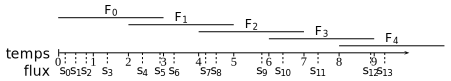
\includegraphics[width=0.7\textwidth]{contrib-astral-fenetres}
	\caption{Séquence de fenêtre de taille $3s$ glissante de $2s$}\label{fig:contrib:astral:fenetres}
\end{figure}

\subsubsection{Fenêtres partitionnées}
L'opérateur de fenêtres partitionnée est très utilisé pour appliquer la même séquences de fenêtres à des sous-flux. Les opérateurs partitionnés sont tous décrit de la même manière. Le principe, illustré dans la figure~\ref{fig:contrib:astral:partition} est de divisé le flux suivant un (ou des) attributs $A$ donné. Sur chacun de ces sous-flux est appliqué un opérateur quelconque. Par la suite, une union est appliquée.
\begin{figure}[ht]
	\centering
	\includegraphics[width=0.9\textwidth]{contrib-astral-partition}
	\caption{Principe d'un opérateur partitionné}\label{fig:contrib:astral:partition}
\end{figure}
\begin{defi}[Séquence de fenêtre partitionnée]
	Soient $S$ un flux, $a_1,...,a_k$ un ensemble d'attributs du schéma de $S$, et $(\alpha,\beta,\gamma)$ une DSF,
	
	Soit $\cup^*$ l'union relationnelle conservatrice des identifiants physiques, 

	Alors la séquence de fenêtre $(\alpha,\beta,\gamma)$ partitionnée par $a_1,...,a_k$ est définie par :
	$$S[a_1...a_k/\alpha,\beta,\gamma] = \mathop{\bigcup\null^*}_{a\in Dom(a_1,...,a_k)} (\sigma_{(a_1,...,a_k)=a} S)[\alpha,\beta,\gamma]$$
\end{defi}

Nous remarquons que nous utilisons la définition conservatrice de l'union relationnelle présenté dans la section précédente, ainsi l'ordre naturel décrit dans le flux d'entrée pourra être retrouvé dans la relation de sortie.
\begin{example}
	L'exemple le plus courant étant la représentation de l'état actuel d'un système à partir d'un flux. Supposons un flux d'entrée $DeviceCPU(deviceId,cpu,\t)$, nous donnant les relevés de charge de processeur. Soit la description de fenêtre rapportant le dernier n-uplet d'un flux : $(1j,1j,1)$. Nous pouvons obtenir la relation temporelle représentant pour chaque dispositif $deviceId$, la dernière valeure connue de $cpu$ et son \textit{timestamp de mesure} $\tau$ : $$DeviceCPU[id/1j,1j,1]$$

	Cet exemple illustre comment nous pouvons passer d'un flux brut à une représentation (dynamique) d'un \textbf{contexte}.
\end{example}

Par la suite, nous utiliserons plusieurs notations simplifiés pour désigner des descriptions de fenêtres courantes décrites dans le tableau~\ref{tab:windows}.
\begin{table}
\centering
\begin{tabular}{c||p{0.4\textwidth}|p{0.4\textwidth}}
  & Définition & Équivalence \\ \bottomrule
 $[L]$ & $[j,j,1]$ &  \\ 
 & \multicolumn{2}{p{0.8\textwidth}}{La séquence de fenêtre où chaque fenêtre ne contient que le dernier n-uplet du flux. Cette séquence est égale à $[B]$ si le flux réparti ses n-uplets avec un n-uplet par \textit{batch}.} \\ \hline
 $[B]$ & $[\tau_S^{-1}(\tau_S(j)^-)+1,j,1]$ & $\{s\in S, \BS(s) = \tau_S\circ\tau_S^{-1}(b)\}$ \\ 
 & \multicolumn{2}{p{0.8\textwidth}}{Séquence de fenêtre où chaque fenêtre contenient le dernier \textit{batch}.} \\\hline
 $[\infty]$ & $[0,j,1]$ & $\{s\in S, \BS(s) \leq b\}$ \\
 & \multicolumn{2}{p{0.8\textwidth}}{Séquence accumulative contenant tout le flux jusqu'au \textit{batch} courant.} \\\hline
 $[T\ r]$ & $[\max(rj-r+t_0,t_0),rj+t_0,r]$ &  \\
 & \multicolumn{2}{p{0.8\textwidth}}{Fenêtre temporelle de taille $r$ se déplaçant toutes les $r$ unités de temps.} \\\hline
 $[P\ r]$ & $[\max(rj-r,0),rj,r]$ &  \\
 & \multicolumn{2}{p{0.8\textwidth}}{Fenêtre positionnelle de taille $r$ n-uplets se déplaçant tous les $r$ n-uplets.} \\
 \toprule
\end{tabular}
\caption{Liste des fenêtres courantes} \label{tab:windows}
\end{table}

Il est important de noter que les équivalences citées sont toutefois non triviales, des démonstrations formelles sont fournies en annexes.

\subsection{Streamers}
\subsection{Domaine}
\subsection{Spread}
\section{Transposabilité}\label{sec:contrib:astral:transposabilite}
La définition de l'équivalence de requête (def~\ref{def:equivalence}) spécifie que les entités sont toutes deux initialisées à un \textit{timestamp} $t_0$. Ce type d'équivalence permet de réécrire une requête avant de l'exécuter tout en conservant exactement le même comportement. Toutefois, cela ne permet pas de comparer avec une requête déjà en exécution, puisque la requête n'est pas synchronisé au même instant. Pour intégrer des données provenant de différentes parties, cet aspect a une grande importance.
\subsection{Équivalence de requêtes multitemporelle}
Pour illustrer l'idée d'effectuer des équivalences de requêtes à différents moments n'est pas trivial, prenons un exemple. Soit la requête $CPU[B]$. Cette requête représente la relation contenant le dernier \textit{batch} du flux \textbf{CPU}. Dans cette requête, durant la période $[t_0,\tau_S(0)[$, par définition, la relation est vide : il est nécessaire d'attendre le premier n-uplet pour former le résultat. Si nous prenons une autre requête ayant démarré au timestamp $t_1 \ll t_0$. Alors pendant la période $[t_0,\tau_S(0)[$, il contient son dernier \textit{batch}. Ceci constitue un exemple de ce que nous appelerons le phénomène d'élaboration défini en~\ref{def:elaboration}.
\begin{defi}[Phénomène d'élaboration]\label{def:elaboration}
    Le phénomène d'élaboration correspond à une période initiale de la vie d'une requête durant laquelle le résultat n'est pas calculable. Cette période transitoire constitue l'élaboration d'une requête.
\end{defi}

Ainsi, nous sommes capable d'établir l'équivalence entre deux requêtes par la définition~\ref{def:equivalencegenerale} qui précise que les résultats sont équivalents à partir d'un certain moment. Pour cela, nous définissons qu'il existe un \textit{timestamp} pour lequel, l'initialisation des entités (grâce à $\sigma$ et $\D$) au ce \textit{timestamp} implique une équivalence des résultats.
\begin{defi}[Équivalence de requêtes générale]\label{def:equivalencegenerale}
    Soient $(Q_1(E_1),t_1)$ et $(Q_2(E_2),t_2)$ deux requêtes quelconques,

    Soit $\E_t$ l'opérateur égal à $\begin{cases} \sigma_{t\geq \t} & \textrm{ si les requêtes sont des flux}\\ \D_{t\geq \t}^{(t,i)} & \textrm{  si les requêtes sont des relations}\end{cases}$

    Alors l'inclusion de requêtes entre ces requêtes est définie par $$\exists t \in \T, \textrm{ tel que } \quad (\E_t\ Q_1(E_1), t_1) \subseteqq (\E_t\  Q_2(E_2), t_2)$$

    L'équivalence de requêtes est définie par double inclusion.
\end{defi}

Nous avons défini une notion générique d'équivalence. Voyons désormais les conséquences du changement de \textit{timestamp} d'initialisation pour une requête donnée.
\subsection{Transposabilité}
La transposabilité telle que définie par la définition~\ref{def:transposabilitereq} est de changer le \textit{timestamp} de départ d'une requête.
\begin{defi}[Transposabilité de requête]\label{def:transposabilitereq}
    Soit $(A,t_0)$ une requête,

    $A$ est transposable par $B$ sur $T\subseteq \T$ si et seulement si : $$\forall t\in T, \quad (A,t_0) \equiv (B,t)$$

    $A$ est dite \textit{naturellement} transposable si $B=A$.
\end{defi}
Toutefois, cette définition ne permet pas de conclure sur l'équivalence de requête car nous ne pouvons pas a priori calculer la transposition de la requête sur son nouveau \textit{timestamp}. Pour permettre la résolution de ce problème, nous allons raisonner par récurrence sur les opérateurs. Comme le défini la définition~\ref{def:transposabiliteop}, chaque opérateur peut se transposer en un autre sur un ensemble de \textit{timestamp} calculé.
\begin{defi}[Transposabilité d'opérateur]\label{def:transposabiliteop}
    Soit $O$ un opérateur unaire,

    Soit $(Q,t_0)$ une requête transposable par $Q'$ sur $E$,

    $O$ est un opérateur transposable par $O'$ sur $T$ si et seulement si : $$(OQ,t_0) \textrm{ est naturellement transposable par } O'Q' \textrm{ sur } T\cap E$$

    $O$ est dit \textit{naturellement} transposable si $O'=O$.
\end{defi}

Il est nécessaire d'initialiser la récurrence en supposant que pour toute expression algébrique, il est possible de trouver un ensemble d'entité source naturellement transposable. Du point de vue de l'implémentation, les sources de données produisent les mêmes flux ou relations quelque soit le moment où elles sont exploitées.
\begin{hyp}[Transposabilité native]\label{hyp:transposabilite}
    Soit $(Q(E),t_0)$ une requête,

    Alors il existe une expression $Q'(E')$ telle que : $$\forall A\in E', \qquad A \textrm{ est naturellement transposable sur } \T$$
    
    Les éléments de $E'$ sont appelés sources de la requête.
\end{hyp}
Cette affirmation reste toutefois à travailler car lors du déploiement d'une requête, nous instantions aussi le processus d'acquisition, qui est lui dépendant du moment de démarrage. Ces aspects sont détaillés lors de l'exploration de l'expressivité d'Astral dans le chapitre~\ref{chap:validation:expressivite}. Afin d'illustrer les propriétés de transposabilité, nous allons montrer la transposabilité d'une requête simple.

\begin{example}\label{ex:transposabilite} 
    Supposons que nous souhaitons obtenir la transposabilité de la requête permettant d'obtenir toutes les 5 secondes la liste des dispositifs actuellement connectés dans la maison : $$\RS{5s} (\sigma_{deviceStatus=1} Devices).$$

    Ici, nous supposons par l'hypothèse des transposabilités des sources que $Devices$ est naturellement transposable à tout instant. La sélection est un opérateur qui a la particularité de ne traiter que l'instant présent et est naturellement indépendant de $t_0$. Ainsi, $\sigma_{deviceStatus=1} Devices$ est naturellement transposable à tout instant.

    Par contre, $\RS{r}$, lui n'est pas transposable à tout moment. En effet, dans sa définition la condition d'appartenance au flux produit est la suivante : $s \in R(t,i)\wedge t-t_0 \equiv 0[r]$. Ainsi, si nous transposons à $t_1$, pour obtenir l'équivalence des requêtes, il est nécessaire que $\forall t \geq t_1$, $t-t_0\equiv t-t_1\equiv 0[r]$.  Ce qui nous conduit à montrer que $t_1 = t_0 +kr$ avec $k\in \Z$. 

    Supposons que $t_1$ vérifie cette condition. Nous arrivons très facilement à voir que $\forall R$, en prenant $t=\max(t_1,t_0)$, nous avons bien\footnote{en suivant naturellement les définitions, nous obtenons de plus une égalité stricte même sur les $\varphi$} que $(\E_{t}\RS{r}(R),t_0) \equiv (\E_{t}\RS{r}(R),t_1)$.
    \begin{center}$\RS{5s}\sigma_{deviceStatus=1} Devices$ est naturellement transposable sur $\{t\in \T /\ t\equiv t_0 [5s]\}$\end{center}
\end{example}

Nous avons désormais montré comment nous pouvions faire des équivalences de requêtes à travers le temps et comment manipuler ces concepts pour en extraire des propriétés. Dans le chapitre~\ref{chap:validation:expressivite}, nous explorons des cas généraux et plus complexe de transposabilité pour démontrer la puissance d'expression d'Astral.

\section{Conclusion}
Après 20 années de recherche, la gestion de flux de données devient désormais suffisamment mature pour être appliqué massivement. Plusieurs produits commerciaux sont d'ailleurs maintenant utilisés en production. Toutefois, nous pouvons nous rendre compte que la complexité théorique de ces systèmes a été sous-estimé. De nombreux modèles ont été décrit pour représenter les flux de données et leurs traitements. Ces modèles sont encore remis en questions aujourd'hui au fur et à mesure des applications concrètes. 

Nous avons vu que le problème d'avoir une bonne connaissance du modèle et du comportement théorique des SGFD est crucial. En l'état, l'intégration des supports persistants reste ad-hoc et assisté par l'utilisateur. Un fonctionnement intégré avec une modélisation générique capable de gérer les deux modes d'interrogations de façon unifiée est donc indispensable pour manipuler correctement flux et relations persistantes. Similairement, les contributions sur l'optimisation de traitement des requêtes sont encore principalement ponctuelles. Afin d'appliquer un traitement efficace pour toute requête, il est nécessaire d'avoir une bonne connaissance théorique du traitement.

Notre contribution technique se concentrera sur trois points principaux :
\begin{itemize}
 \item[\textbf{Modélisation}] : Création d'Astral, algèbre de traitement des requêtes continues sur flux et relations temporelles. Nous accorderons de l'importance sur la prise en compte des problèmes relevés en section~\ref{sec:rw:sgfd:modeles:synthese}. Cette algèbre sera présenté dans le chapitre~\ref{chap:contrib:astral}
 \item[\textbf{Exécution}] : Mise en œuvre de l'intergiciel Astronef pour construire et exécuter efficacement une requête exprimée avec l'algèbre Astral. Ainsi, à partir d'une requête algébrique, il est possible de sélectionner le plan de requête qui semble le plus efficace grâce aux connaissances accumulés. Cette mise en œuvre sera développée dans le chapitre~\ref{chap:contrib:execution}.
 \item[\textbf{Persistance}] : Conception de l'extension Asteroid permettant l'intégration des requêtes continues sur flux et des requêtes sur support relationnel persistant. Ceci permettra de gérer la représentation du système observé ainsi que l'historisation des données dynamiques. Le support mathématique de cette intégration sera supporté par Astral et sa mise en œuvre par Astronef. Cette intégration sera effectuée dans le chapitre~\ref{chap:contrib:persistance}.
\end{itemize}

Grâce à ces contributions, il deviendra possible de mettre en œuvre un système d'observation générique applicable sur tout type de données. L'utilisateur devra exprimer des requêtes dans le langage algébrique Astral. Une fois ces requêtes écrites, nous serons garanti de leur mise en œuvre. Le tableau~\ref{tab:rw:contrib} résume l'ensemble des points d'analyses que nous nous étions fixés en section~\ref{sec:rw:supervision:criteres}.
\begin{table}[!ht]
\criteretabDonnee
    {Relationnel dérivé. Nous réutilisons les principes utilisés dans la gestion de flux et des bases de données.}
    {\good Modèle entité-relation augmenté pour supporter les flux.}
    {\good Requêtes sur tout type de données (flux, relations).}
\criteretabTraitement
    {\good Continue, Instantannée, Mixte}
    {\good Utilisation des requêtes continues des SGFD en tant qu'intégrateur.}
    {\meh Astral : langage de requête algébrique. Un langage purement déclaratif reste toutefois dérivable de ces fondations théoriques.}
    {\good Relationnel avec support \textbf{intégré} du dynamisme des données.}
\criteretabAdaptabilite
    {\good Spécification du modèle du système ainsi que des requêtes d'intégration (algébriques).}
    {\meh Pour l'analyse, la gestion de données multi-dimensionnelles des entrepôts utilisés est utilisé. Pour l'interrogation continue, utilisation d'un opérateur de préférences sur les flux.}
    {\good Infrastructure générique capable de supporter l'ajout d'opérateurs avec plusieurs implémentations.}
    {\good Héritage de l'efficacité des flux de données. Sélection du meilleur plan d'exécution pour chaque requête. Héritage des supports de grands volumes grâce aux entrepôts.}
\caption{Résumé de notre contribution selon nos critères}\label{tab:rw:contrib}
\end{table}

\begin{savequote}[6cm]
<< If you will remember back,\\ The words I spoke were quite exact. >>
\qauthor{Zecora}
\end{savequote}

\chapter{Expressivité d'Astral}\label{chap:validation:expressivite}
\chaptertoc

\section{Choix des fondations de l'algèbre}\label{sec:valid:expressivite:modele}
Lors de l'établissement des premières définitions d'Astral dans la section~\ref{sec:contrib:astral:definitions}, nous avons fait des choix concernant le temps, les entités et les équivalences de requêtes. Cette section discute de la validité de ces choix par en montrant que des choix différents auraient menés à des ambiguïtés sémantiques. Nous présentons d'abord l'hypothèse de continuité du temps. Nous analysons ensuite nos choix en terme de gestion des ordres. Enfin, nous détaillons les équivalences de requêtes.

\subsection{Continuité du temps}
La définition~\ref{def:timestamp} présente un \textit{timestamp} en tant qu'élément d'un espace continu. Nous avons vu que dans la littérature, le temps était souvent considéré comme un entier, ou au mieux dans un espace isomorphe à $\N$. Ce choix permet de mieux gérer les différences d'interprétation du temps par l'implémentation.

En effet, chaque système informatique est limité par un \textit{chronon} : la plus petite différence de timestamp observable. Pour certains système, ce \textit{chronon} est d'une milliseconde, d'autres d'une seconde et d'autres d'un \textit{tick} processeur. Ne pas se restreindre à un \textit{chronon} particulier nous permet de manipuler facilement les \textit{timestamps} issus de deux systèmes de datation (synchronisés) sans ambiguïté. De façon plus formelle, nous aurions pu définir le temps comme un ensemble isomorphe à $\N$ quelconque mais les jointures et autres opérations binaires auraient été plus complexe.

Nous remarquons aussi que ce choix nous a permis de clarifier l'opérateur $\mathcal{RS}$ de STREAM~\cite{Arasu:stream}. Cet opérateur est décrit par la phrase \enquote{\it à chaque timestamp, envoyer l'ensemble de la relation}. Nous avions potentiellement une ambiguïté sachant que l'interprétation de \textit{timestamp} pouvait dépendre du système dans lequel il était exécuté. Cet opérateur est remplacé par $\RS{r}$ dans Astral avec $r$ une période de temps explicite.

\subsection{Hypothèse de la cohérence temporelle}
L'hypothèse de la cohérence temporelle~\ref{hyp:ordres} affirme que les n-uplets doivent arriver dans un flux de manière ordonnée selon leurs \textit{timestamps}. Cette hypothèse a suscité beaucoup d'intérêt de la part de la communauté. La question ouverte est de savoir s'il est nécessaire que des opérateurs existent dans l'algèbre, ou est-ce à l'implémentation de le garantir d'une manière ou d'une autre ? Nous pouvons par exemple noter Aurora~\cite{Abadi:aurora} qui avait défini des opérateurs spécifiques au réordonnement d'un flux grâce à une mémoire tampon de $n$ n-uplets.

En supposant que l'hypothèse n'est pas vérifiée, nous avons la fonction position-\textit{batch} (def~\ref{def:tau}) qui n'est plus croissante. Ainsi, sa pseudo-inverse n'existe plus, ce qui fait qu'il devient impossible de définir les séquences de fenêtres telles que nous les avons faites. Il est, en effet, facile de voir que la fenêtre explicitant les $50$ derniers n-uplets. La notion de dernier est sémantiquement lié aussi à son \textit{timestamp} ce qui induit des confusions. D'un point de vue implémentation, la croissance du temps fait qu'une fois qu'un \textit{timestamp} $t$ est présent dans un n-uplet, nous sommes garanti que toutes les données inférieures à $t$ sont arrivées. Ainsi le \textit{scheduler} peut décider d'exécuter un opérateur en garantissant son résultat.

Notre constat est le suivant : pour avoir une algèbre sans ambiguïté sémantique, nous devons supposer que les \textit{timestamps} sont croissants. C'est à l'implémentation de garantir cette contrainte, et si elle n'est pas vérifiée, il devient très difficile de prévoir les conséquences que cela va induire.

\subsection{Sémantiques d'ordres}
L'évaluation d'une relation temporelle à un \textit{batch} donné n'est pas un ensemble d'n-uplet, c'est une séquence. Ce choix est central car il intervient dans la majorité des définitions. Que ce soit dans la définition du produit cartésien~\ref{def:produit} ou des \textit{streamers}~\ref{def:streamers}, nous explicitons la sémantique que nous choisissons pour l'ordre des n-uplets résultants.

Dans la littérature, les flux sont souvent étendus du modèle $\mathcal{SEQ}$~\cite{Seshadri:seq} décrivant les manipulations de séquences. Il est acquis que les flux sont des ensembles totalement et strictement ordonnés. Or, lorsque nous transformons ce flux en relation temporelle, cet ordre est rarement abordé. Pourtant, nous avons vu dans la définition des \textit{streamers}~\ref{def:streamers} qu'il faut assigner un ordre strict aux flux produits. 

Dans Astral, nous considérons que les relations instantanées doivent avoir un ordre pour obtenir un flux correctement ordonné après l'application d'un \textit{streamer}. Ainsi, nous n'avons pas d'ambiguïté sémantique lié à cet aspect. Cette formalisation plus stricte nous a amené à découvrir le théorème~\ref{thm:asymetrie} qui dévoile l'asymétrie du produit cartésien, contrairement aux affirmations actuelles.

Il est important de noter que ce théorème est vrai à cause du choix de l'équivalence de requête (def~\ref{def:equivalence}). Cette équivalence inclue deux notions, celle des entités initialisé qui prend tout son sens dans le cadre des transpositions, et celle des inclusions et équivalences de séquences. Nous avons en effet définit l'inclusion des relations instantanées comme une définition d'inclusion de suite, ce qui nécessite une équivalence de l'ordre. Une définition différente de l'équivalence de requête permettrait d'obtenir une symétrie du produit. Dans la pratique, il est en effet possible que l'utilisateur souhaite obtenir ses n-uplets dans un ordre quelconque, ce qui pourrait permettre des optimisations supplémentaires.

Nous avons présenté comment les choix que nous avons fait pour les fondations de l'algèbre permettent d'avoir une sémantique claire et sans ambiguïté. Nous comparons maintenant l'expressivité d'Astral comparé aux algèbres existantes.
\section{Comparaison de l'expressivité d'Astral}\label{sec:valid:expressivite:comparaison}
L'algèbre Astral a été conçue pour permettre d'exprimer des requêtes continues sans ambiguïté, mais aussi pour introduire de nouveaux opérateurs afin d'étendre la puissance d'expression des requêtes continues. Dans cette section, nous analysons en détail son expressivité. En premier lieu, nous détaillons qu'Astral couvre naturellement un large ensemble des approches actuelles. Ensuite, nous analysons les opérateurs que nous avons particulièrement remodelés : les séquences de fenêtres et la manipulation temporelle.

\subsection{Expressivité générale}
Astral est inspiré de l'algèbre \textit{ACO} de \textit{STREAM}. Nous avons repris la majeure partie des idées, notamment celle d'avoir des flux et des relations, et avons appliqués nos définitions plus strictes, comme nous l'avons vu dans la section précédente. Nous pouvons affirmer que nous couvrons l'expressivité de \textit{STREAM}.

Sachant que \textit{STREAM} a démontré dans~\cite{Arasu:stream} que son expressivité couvre les approches de l'époque comme \textit{Chronicles}, \textit{Tribeca}, \textit{NiagaraCQ} ou \textit{Aurora}. Nous pouvons considérer qu'Astral est, par transitivité, plus expressive que ces travaux.

Notre formalisation à base de \textit{batch} nous permet de supporter les sémantiques exposées par~\cite{Jain:spread}. Nous avons de même présenté notre interprétation des opérateurs \textit{SPREAD} correspondant aux définitions décrites. Il est toutefois notable que les parties où les auteurs spécifiaient des choix non-déterministes ont été remplacés par des choix sur l'ordre positionnel.

Nous avons vu que Astral couvrait une grande partie des approches actuelles. Nous allons maintenant nous concentrer sur l'opérateur le plus étudié de la littérature : les séquences de fenêtres.

\subsection{Fenêtres}
Dans cette section, nous analysons l'expressivité des séquences de fenêtres. Afin de voir les capacités de notre formalisation, nous revisitons les expressions de fenêtres présentés dans l'état de l'art. Nous commençons par la sémantique la plus largement utilisé de la fenêtre glissante \textit{RANGE}/\textit{SLIDE}.
\subsubsection{RANGE $x$ SLIDE $y$}
Dans le cadre de la fenêtre glissantes, il existe deux descriptions possibles. La définition exacte telle que présente dans plusieurs travaux et telle que spécifiée dans~\cite{Jain:spread} est la suivante :

\DSF{r = y}{\beta(j) = yj+t_0}{\alpha(j) = \max(yj-x,0)+t_0}

Comme spécifié, les premiers états des bornes ont une largeur de fenêtre plus petite que $x$. Dès que $j \geq \frac xy$, alors la largeur temporelle deviendra égale à $x$. Nous pouvons noter que la fonction $\alpha(j) = yj-x+t_0$ n'est pas valide dans notre contexte. La seconde condition des DSF (def~\ref{def:dsf}) nécessite $\alpha \geq t_0$, ce qui n'est pas vraie pour $i=0$. L'insertion de la fonction $\max$ rend la description viable et décrit la sémantique des premières phases, ce qui n'est pas explicite dans sa description textuelle.

La description suivante est aussi valide, mais ne possède pas de phase initiale. Ici, la relation temporelle est vide jusque $\beta(0)$ afin d'assurer que la fenêtre couvre toujours une largeur temporelle de $x$.

\DSF{r = y}
	{\beta(j) = yj+x+t_0}
	{\alpha(j) = yj+t_0}

Afin d'illustrer les différences entre les deux sémantiques possibles, la figure~\ref{fig:valid:expressivite:slidemax} représente les différences d'évaluations pour une fenêtre glissante avec $y=2$ et $x=4$. Dans le premier cas ($\max$), il y a deux autres évaluations à $i=0$ et $i=1$. Après cette partie, comme démontré précédemment les deux modèles sont identiques.

\begin{figure}[ht]
\centering
\def\lgrad#1{\draw [thick] (#1,0) -- (#1,-0.2); \node [below] at (#1,-0.2){#1};}
\def\seg#1#2#3#4#5{\draw [thick] (#1#40.1,#3+0.25) -- (#1,#3+0.25) -- (#1,#3-0.25) -- (#1#40.1,#3-0.25); \draw [thick] (#1,#3) -- (#2,#3); \draw [thick] (#2#50.1,#3+0.25) -- (#2,#3+0.25) -- (#2,#3-0.25) -- (#2#50.1,#3-0.25);}
\def\seglbl#1#2#3#4#5#6{\seg{#1}{#2}{#3}{#4}{#5}\node [above] at (0.5*#1+0.5*#2,#3){#6};}
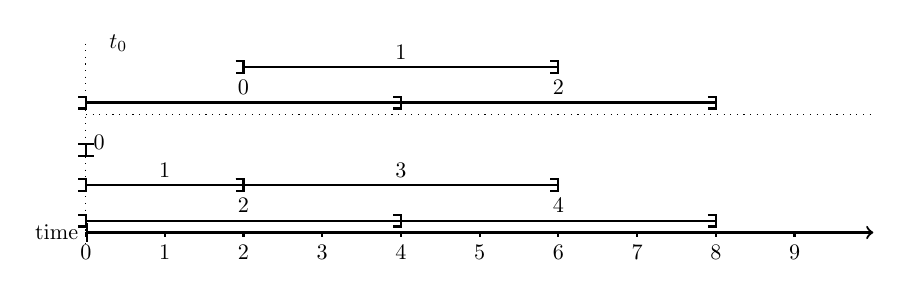
\begin{tikzpicture}[xscale=1, yscale=0.3, every node/.style={scale=0.8}]
\node [left] at (0,0) {time};
\draw [thick,|->] (0,0) -- (10,0);

\seg{0}{0}{3.5}-+\node [right] at (0,3.8){0};
\seglbl{0}{2}{2}--{1};
\seglbl{0}{4}{0.5}--{2};
\seglbl{2}{6}{2}--{3};
\seglbl{4}{8}{0.5}--{4};
\draw [dotted] (0,8) -- (0,-0.5); \node [right] at (0.2,8) {$t_0$};

\seglbl{4}{8}{5.5}--{2};
\seglbl{2}{6}{7}--{1};
\seglbl{0}{4}{5.5}--{0};
\draw [dotted] (0,5) -- (10,5);
\lgrad{0} \lgrad{1} \lgrad{2} \lgrad{3} \lgrad{4} \lgrad{5} \lgrad{6} \lgrad{7} \lgrad{8} \lgrad{9} 
\end{tikzpicture}
\caption{Différence entre les sémantiques avec ou sans $\max$ dans la description RANGE 4 SLIDE 2}\label{fig:valid:expressivite:slidemax}
\end{figure}

Nous pouvons remarquer que nous avons aussi introduit la notion d'inclusion de bornes. Ce qui permet de clarifier si la borne inférieure est incluse dans le contenu de la fenêtre. Dans le cadre des fenêtres glissantes ce n'est pas le cas~\footnote{Il est intéressant de noter un erratum dans la spécification de cet opérateur où la définition précise que la borne inférieure est incluse alors que les exemples et les expérimentations pratiques indiquent le contraire.}.

\subsubsection{RANGE $x$}
Dans ses définitions usuelles, RANGE $x$ seule est possible et est similaire à RANGE $x$ SLIDE 1. Dans Astral, le temps n'est pas discret et une telle définition n'a pas de sens. Une définition similaire est possible en supposant que le \textit{chronon} du système d'implémentation est $\varepsilon$, alors : RANGE $x$ = RANGE $x$ SLIDE $\varepsilon$.

Une approche plus propre serait d'utiliser une DSF générique en basant ses instants d'évaluations (fournis par $\gamma$, pour rappel) sur les arrivés et départs d'n-uplets dans la fenêtre. Toutefois une connaissance de $\alpha^{-1}$ et $\beta^{-1}$ est nécessaire et rend son expression plus complexe. Il est intéressant de voir que ce comportement est telle qu'implémenté car un opérateur vérifiant à chaque \textit{timestamp} système si un n-uplet doit sortir de la fenêtre n'est pas efficace. Il est plus efficace de planifier (via le \textit{scheduler}) ses instants d'évaluations.

\subsubsection{Descriptions à bornes linéaires}
Dans SStreamWare~\cite{Gurgen:sstreamware}, les fenêtres sont définies par un 5-uplet (start, end, rate, start\_adv, end \_adv) :
\begin{itemize}
	\item start (resp. end) décrit la borne inférieure (resp. supérieure) de la première fenêtre produite par la séquence
	\item rate est la fréquence d'évaluation
	\item start\_adv (resp. end\_adv) décrit la quantité de glissement de la borne inférieure (resp. supérieure) à chaque évaluation.
\end{itemize}

Dans Astral, ce comportement est facilement représentable sous forme de DSF :
\DSF{r = \textrm{rate}}
	{\beta(j) = \textrm{end\_adv}*j+\textrm{end}}
	{\alpha(j) = \textrm{start\_adv}*j+\textrm{start}}

\subsubsection{Descriptions procédurales}
Dans les premières versions de TelegraphCQ~\cite{Chandrasekaran:telegraphcq}, les descriptions de fenêtres étaient faites par une boucle \textit{for} procédurale sur un \textit{timestamp} :
\begin{lstlisting}[language=C]
for(t = init ; continue(t) ; t = evolution(t))
	WindowIs(S, begin(t), end(t))
\end{lstlisting}

Ceci peut être formalisé grâce à une DSF générique. Considérons la suite suivante : $u_0=$ init, $u_n=$ evolution($u_{n-1}$) si continue($u_{n-1}$) est vraie, $u_n = u_{n-1}$ sinon. Alors, nous obtenons la description suivante :

\DSF{\gamma(t,i) = \displaystyle\sum_{i=0}^{+\infty} u_i \indic_{[u_i, u_{i+1}[}(t)}
	{\beta = \textrm{end}}
	{\alpha = \textrm{begin}}

La fonction $\gamma$ est définie par une liste de points. Cette définition est courante pour les définitions des fonctions en escaliers. Il est notable que pour des fenêtres avec un taux d'évaluation constant et une position initiale usuelle, une DSF simplifiée est suffisante. 
\subsubsection{Description multi-domaines}
Dans certains systèmes d'observations~\cite{Jurdak:sumac}, il est courant de récupérer les données par vague. Ainsi, dans les interfaces d'observations, nous pouvons régulièrement voir des séquences de fenêtres \enquote{les $n$ derniers n-uples toutes les $m$ secondes}. Pour formaliser une telle séquence, il n'est pas nécessaire d'utiliser une DSF générique car l'évaluation reste périodique. Voici la description de la séquence précédemment décrite :

\DSF{r=m}
	{\beta(j) = \rtau(mj+t_0)}
	{\alpha(j)= \max(\rtau_S(mj+t_0)-n,0)}

Le taux est temporel et les bornes sont positionnelles. Le pont entre les domaines est assuré par l'opérateur grâce aux fonctions $\tau_S$ et $\rtau_S$. Dans ce cas, l'expression $\rtau_S(mi+t_0)$ donne la position à un \textit{timestamp} donné. La remarque concernant le $\max$ que nous avions faite plus tôt reste valable ici.

\subsubsection{Introduction d'un délai}
Dans les travaux de Patroumpas et Sellis~\cite{Patroumpas:window}, l'introduction d'un délai de traitement a été formalisée. En effet, si un n-uplet possède un \textit{timestamp} légèrement déphasé par rapport à son temps réel, alors la fenêtre peut tout de même l'inclure.

Sa formalisation dans notre cas revient à légèrement changer notre fonction $\gamma$ par $\gamma'$ qui décale l'évaluation de $\delta$. Par exemple, nous obtenons pour une description temporelle : $$\gamma'(t,i) = \gamma(t-\delta,i) = \left\lfloor\frac{t-\beta(0)-\delta}{r}\right\rfloor$$

\subsubsection{Modèle d'exécution de SECRET}
Enfin, SECRET~\cite{Botan:secret} est un modèle permettant de généraliser les sémantiques d'exécutions des fenêtres. L'approche est de découper l'exécution d'une fenêtre en quatre concepts que nous pouvons retrouver dans Astral.
\begin{itemize}
	\item Les \textit{Ticks} décident du moment où le système doit réagir au flux (sémantique basé n-uplet, basé temps ou \textit{batch}).
	\item Le \textit{Content} défini le contenu global de la fenêtre par son \textit{Scope}, c'est à dire sa description.
	\item Enfin, un \textit{Report} envoie le résultat final.
\end{itemize}

Bien que les approches soient différentes : nous retrouvons des notions similaires. Le \textit{Scope} est similaire à $\alpha$, $\beta$. Le \textit{Content} à une fenêtre en particulier. Les \textit{Ticks} et les \textit{Reports} sont faites grâce à la fonction $\gamma$ et le contrôle du mode d'exécution par les opérateurs \textit{SPREAD}. L'avantage de l'approche de SECRET est de pouvoir qualifier rapidement le comportement de l'exécution d'un SGFD en particulier, alors qu'Astral décrit la sémantique exacte du résultat pour l'utilisateur.

Nous avons désormais détaillé le positionnement de l'opérateur de séquence de fenêtre par rapport à la littérature. Nous constatons que l'opérateur permet de couvrir l'ensemble des sémantiques actuellement découvertes. Nous avons clarifié plusieurs descriptions non-triviales telles que les fenêtres RANGE stricte, les fenêtres multi-domaines et l'introduction du délai. Nous présentons maintenant l'analyse de l'opérateur de manipulation temporelle.

\subsection{Manipulation temporelle}
L'opérateur de manipulation temporelle (def~\ref{def:manipulation}) permet de transformer le temps \textit{courant} en un temps passé. Ceci permet de transformer le moment d'évaluation de la relation temporelle. Dans l'état actuel de l'art, à notre connaissance, il n'existe pas d'opérateur capable de faire explicitement cette opération. Dans notre cas, il a permit à Asteroid de manipuler facilement la sémantique de mise à jour des relations issues d'un SGBD.

Cet opérateur nous a permit notamment d'introduire la jointure semi-sensible $\ssjoin$. Cette jointure permet de refléter un comportement qui se retrouve dans plusieurs SGFD : ne réagir que sur les mises à jours d'une seule branche.

Une autre application intéressante de cet opérateur est le calcul de changement d'une relation temporelle. Comme nous l'avons vu, l'opérateur $\IS$ est capable de fournir les nouveaux n-uplets d'une relation. Nous pouvons toutefois avoir un résultat pouvant être très intéressant dans le cadre l'observation de système : \enquote{A partir d'une relation temporelle $R$($id$,$v$), fournir le flux des changements ($id$,$v$,$v_{old}$) avec $v_{old}$ l'ancienne valeur pour l'identifiant $id$}. Cette requête s'écrit ainsi :
$$\IS(R \Join_{v\neq v_{old}} (D^{(t,i)^-}_{t>t_0}\rho_{v_{old}/v} R))$$
L'opérateur $D^{(t,i)^-}_{t>t_0}$ retarde la relation temporelle d'un \textit{batch}. Il devient possible d'interroger à un instant donné, une relation temporelle et son état précédent.

Nous avons présenté l'ensemble des aspects novateurs des définitions d'Astral. Nous détaillons maintenant les manipulations possibles grâce à cette algèbre avec un ensemble de propositions et de théorèmes.
\section{Propositions et théorèmes}
\subsection{Commutativité et associativité}
Tableau de projection et de sélection

Associativité de la jointure

Manipulation temporelle

\subsection{Transmission du temps}
Le théorème

Le corrolaire fondamental

\subsection{Transposabilité}
Transposabilités simples

Théorème général des fenêtres

Application au cas linéaire

\subsection{À la recherche du cœur}
A voir si on a des trucs sympa... sinon on vire on a assez
\section{Conclusion}
Après 20 années de recherche, la gestion de flux de données devient désormais suffisamment mature pour être appliqué massivement. Plusieurs produits commerciaux sont d'ailleurs maintenant utilisés en production. Toutefois, nous pouvons nous rendre compte que la complexité théorique de ces systèmes a été sous-estimé. De nombreux modèles ont été décrit pour représenter les flux de données et leurs traitements. Ces modèles sont encore remis en questions aujourd'hui au fur et à mesure des applications concrètes. 

Nous avons vu que le problème d'avoir une bonne connaissance du modèle et du comportement théorique des SGFD est crucial. En l'état, l'intégration des supports persistants reste ad-hoc et assisté par l'utilisateur. Un fonctionnement intégré avec une modélisation générique capable de gérer les deux modes d'interrogations de façon unifiée est donc indispensable pour manipuler correctement flux et relations persistantes. Similairement, les contributions sur l'optimisation de traitement des requêtes sont encore principalement ponctuelles. Afin d'appliquer un traitement efficace pour toute requête, il est nécessaire d'avoir une bonne connaissance théorique du traitement.

Notre contribution technique se concentrera sur trois points principaux :
\begin{itemize}
 \item[\textbf{Modélisation}] : Création d'Astral, algèbre de traitement des requêtes continues sur flux et relations temporelles. Nous accorderons de l'importance sur la prise en compte des problèmes relevés en section~\ref{sec:rw:sgfd:modeles:synthese}. Cette algèbre sera présenté dans le chapitre~\ref{chap:contrib:astral}
 \item[\textbf{Exécution}] : Mise en œuvre de l'intergiciel Astronef pour construire et exécuter efficacement une requête exprimée avec l'algèbre Astral. Ainsi, à partir d'une requête algébrique, il est possible de sélectionner le plan de requête qui semble le plus efficace grâce aux connaissances accumulés. Cette mise en œuvre sera développée dans le chapitre~\ref{chap:contrib:execution}.
 \item[\textbf{Persistance}] : Conception de l'extension Asteroid permettant l'intégration des requêtes continues sur flux et des requêtes sur support relationnel persistant. Ceci permettra de gérer la représentation du système observé ainsi que l'historisation des données dynamiques. Le support mathématique de cette intégration sera supporté par Astral et sa mise en œuvre par Astronef. Cette intégration sera effectuée dans le chapitre~\ref{chap:contrib:persistance}.
\end{itemize}

Grâce à ces contributions, il deviendra possible de mettre en œuvre un système d'observation générique applicable sur tout type de données. L'utilisateur devra exprimer des requêtes dans le langage algébrique Astral. Une fois ces requêtes écrites, nous serons garanti de leur mise en œuvre. Le tableau~\ref{tab:rw:contrib} résume l'ensemble des points d'analyses que nous nous étions fixés en section~\ref{sec:rw:supervision:criteres}.
\begin{table}[!ht]
\criteretabDonnee
    {Relationnel dérivé. Nous réutilisons les principes utilisés dans la gestion de flux et des bases de données.}
    {\good Modèle entité-relation augmenté pour supporter les flux.}
    {\good Requêtes sur tout type de données (flux, relations).}
\criteretabTraitement
    {\good Continue, Instantannée, Mixte}
    {\good Utilisation des requêtes continues des SGFD en tant qu'intégrateur.}
    {\meh Astral : langage de requête algébrique. Un langage purement déclaratif reste toutefois dérivable de ces fondations théoriques.}
    {\good Relationnel avec support \textbf{intégré} du dynamisme des données.}
\criteretabAdaptabilite
    {\good Spécification du modèle du système ainsi que des requêtes d'intégration (algébriques).}
    {\meh Pour l'analyse, la gestion de données multi-dimensionnelles des entrepôts utilisés est utilisé. Pour l'interrogation continue, utilisation d'un opérateur de préférences sur les flux.}
    {\good Infrastructure générique capable de supporter l'ajout d'opérateurs avec plusieurs implémentations.}
    {\good Héritage de l'efficacité des flux de données. Sélection du meilleur plan d'exécution pour chaque requête. Héritage des supports de grands volumes grâce aux entrepôts.}
\caption{Résumé de notre contribution selon nos critères}\label{tab:rw:contrib}
\end{table}

\chapterhead{Tables de l'algèbre Astral}
\listofdefifloat
\listofthmfloat
\listofpropfloat
\listofcorofloat

